\documentclass[tikz,border=10pt]{standalone}
\usepackage{tikz}
\usetikzlibrary{arrows.meta,positioning}

\tikzset{
  card/.style={draw=blue!70!black, line width=1.2pt, rounded corners=3pt, minimum width=5.0cm, minimum height=1.0cm, align=center, fill=none},
  result/.style={draw=orange!80!black, line width=1.2pt, rounded corners=3pt, minimum width=5.0cm, minimum height=1.0cm, align=center, fill=none},
  flow/.style={-{Stealth[length=3mm]}, line width=1.2pt, draw=black!70}
}

\begin{document}
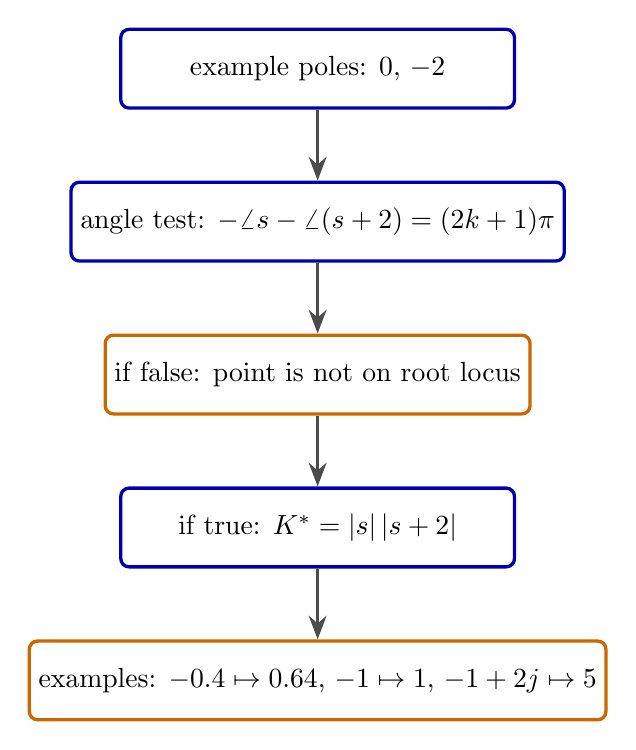
\begin{tikzpicture}[node distance=0.9cm]
  \node[card] (a) {example poles: $0$, $-2$};
  \node[card, below=of a] (b) {angle test: $-\angle s-\angle(s+2)=(2k+1)\pi$};
  \node[result, below=of b] (c) {if false: point is not on root locus};
  \node[card, below=of c] (d) {if true: $K^\ast=|s|\,|s+2|$};
  \node[result, below=of d] (e) {examples: $-0.4 \mapsto 0.64$, $-1 \mapsto 1$, $-1+2j \mapsto 5$};

  \draw[flow] (a) -- (b);
  \draw[flow] (b) -- (c);
  \draw[flow] (c) -- (d);
  \draw[flow] (d) -- (e);
\end{tikzpicture}
\end{document}
